\chapter{Microservices Design Components}
Figure \ref{fig:microarchitecture} shows the microservices components that make up the design of \ac{RAILS}.

\begin{figure}[H]
	\centering
		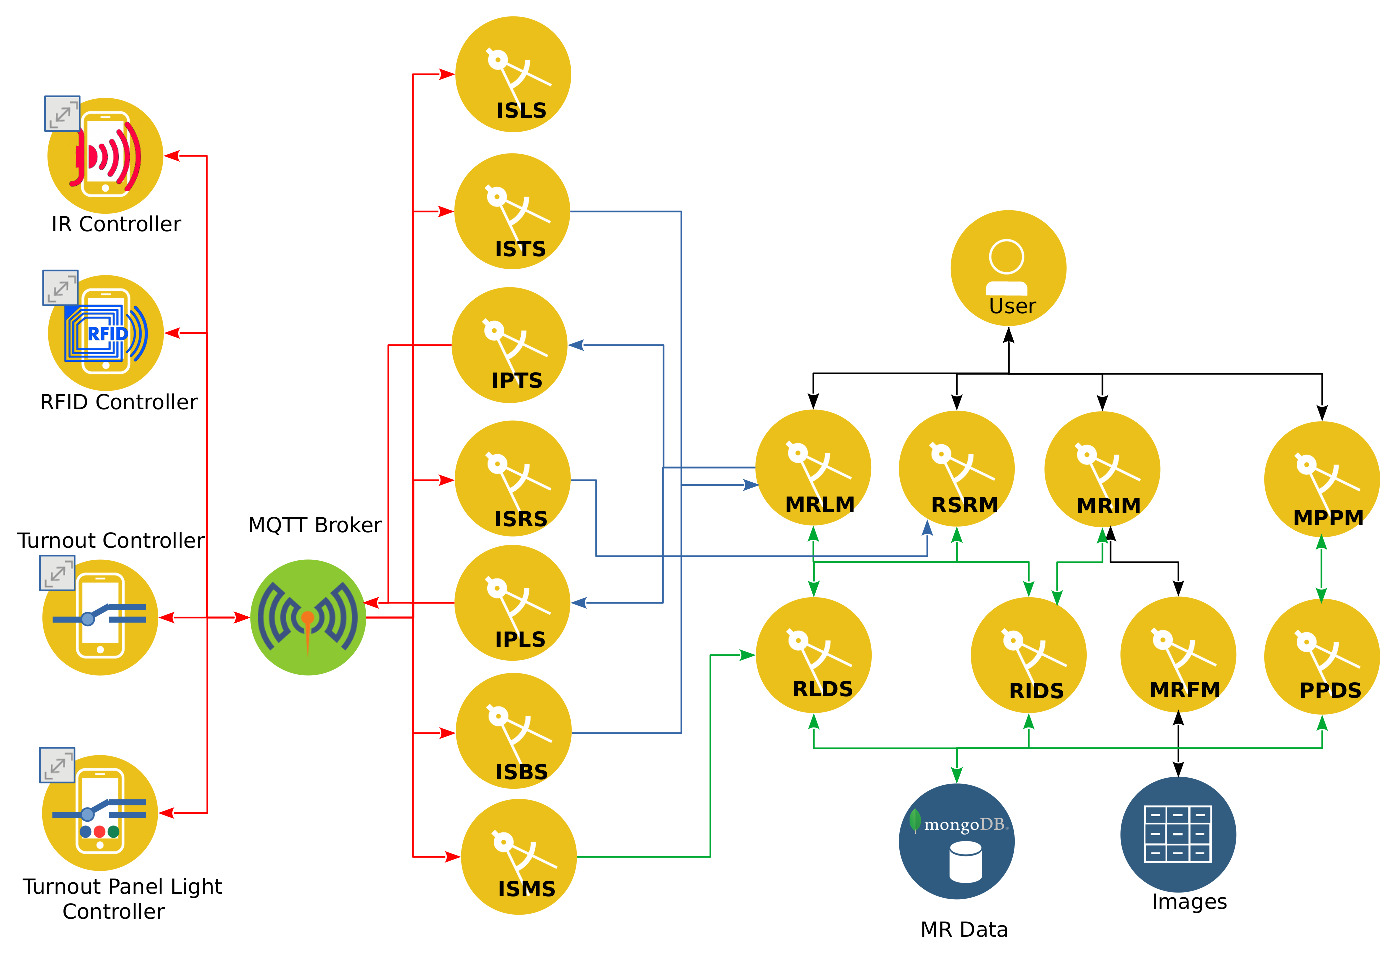
\includegraphics[scale=0.7]{design.eps}
	\caption{Microservices Component Architecture}
	\label{fig:microarchitecture}
\end{figure}

The microservices design components are divided into three sets:
\begin{itemize}
  \item \ac{IoT} components
  \item \ac{DS} components
  \item \ac{SPA} components
\end{itemize}

\section{\ac{IoT} Components}
The components of the \ac{IoT} set of design components are subdivided into:
\begin{itemize}
  \item Micro Controllers using the \ac{MQTT} protocol:
\begin{itemize}
  \item \ac{RFID} Controller processes \ac{RFID} tags obtained from a \ac{RFID} reader and then publishes the value
  \item Turnout Controller subscribes to turnout commands then to act on the command to cause the turnout to move. It then publishes the state of the turnout
  \item \ac{IR} Controller (in planning) processes \ac{IR} sensors and publishes their values
\end{itemize}
  \item \ac{MQTT} Broker is the heart of any publish/subscribe protocol, is responsible for receiving messages, posting to designated topics and sending messages to clients subscribing to topics.
  \item The subscribers and publishers bridge the \ac{MQTT} elements with the \ac{GUI} applications:
\begin{itemize}
  \item \ac{IPLS} publishes turnout panel light commands a Turnout Panel Controller
  \item \ac{IPTS} publishes turnout commands to a Turnout Controller
  \item \ac{ISBS}  subscribes to push button events and pushes them via a web-socket to the MRLM component
  \item \ac{ISLS} (in planning) \ac{IoT} subscribes to topics that provide location information i.e., \ac{IR} Sensors and \ac{RFID} sensors
  \item \ac{ISMS} subscribes to micros and adds or updates micros collection in RAILS. It also subscribes to micro heartbeats.
  \item \ac{ISRS} subscribes to \ac{RFID} tags and pushes them via a web-socket to the \ac{RSRM} component
  \item \ac{ISTS} subscribes to turnout switch closures and pushes them via a web-socket to the \ac{MRLM} component
\end{itemize}
\end{itemize}
\section{\acl{DS} Components}
\ac{DS} consist of all the components that handle and or store the model railroad data:
\begin{itemize}
  \item MR Data – the document repository, MongoDB, to store complete collections of items such as rolling stock, industries (producers and consumers), track elements, turnouts, projects, purchases, etc.
  \item \ac{RIDS} provides REST access to railroad inventory documents
  \item \ac{PPDS} provides REST access to model railroad projects and purchases documents
  \item \ac{RLDS} provides REST access to model railroad layout documents
  \item \ac{MRFM} provides the user the ability to upload image files for the use by the \ac{MRIM} component
  \item Images is the file store for the images uploaded by \ac{MRFM} component and used by the \ac{MRIM} component
\end{itemize}
\section{\acl{SPA} Components}
\ac{GUI} applications that provide user access to RAILS:
\begin{itemize}
  \item \ac{RSRM}, this \ac{SPA} allows a user to match a RFID value to a rolling stock road name and number
  \item \ac{MRIM}, this \ac{SPA} allows a user to create, update and delete model railroad assets, such as rolling stock
  \item \ac{MPPM}, this \ac{SPA} allows a user to enter information about their projects and purchases
  \item \ac{MRLM}, this \ac{SPA} allows a user to enter information about their layout and control elements of it
\end{itemize}
